% !TeX program = pdflatex
%==============================================================================
%  Aula E1 --- Análise de Agrupamento: k-Médias
%  VERSÃO DO ALUNO: texto para leitura autônoma, fora da sala.
%  (O roteiro de sala é "E1 Analise de Agrupamento k-Medias.tex".)
%==============================================================================
\documentclass[11pt,a4paper]{article}
\usepackage[aluno]{../../recursos/latex/estilo-notas}

\title{}
\date{}

\begin{document}
\cabecalhoaula{Extra E1}{Análise de Agrupamento: $k$-Médias}{AME cap.~11; ISLP §12.4}

%==============================================================================
\section*{O que você vai aprender}
%==============================================================================
Ao final desta aula você deve ser capaz de:
\begin{itemize}[leftmargin=1.4cm]
  \item distinguir aprendizado supervisionado de \emph{não supervisionado} e dizer
        por que a avaliação fica mais difícil;
  \item escolher uma medida de \emph{dissimilaridade} e entender que essa escolha
        define o que é um ``grupo'';
  \item enunciar o objetivo do \textbf{$k$-médias} (WCSS) e executar o
        \textbf{algoritmo de Lloyd};
  \item explicar por que Lloyd converge, e para o quê;
  \item escolher $K$ pelo \emph{cotovelo} e pela \emph{silhueta}, sabendo dos
        limites de ambos;
  \item descrever o \textbf{agrupamento hierárquico} e o papel do \emph{linkage}.
\end{itemize}

\noindent
Viramos a chave para o Bloco~III: aqui \textbf{não há rótulos} $Y$. O objetivo deixa
de ser ``prever'' e passa a ser ``descobrir estrutura''. Isso muda tudo, a começar
pela pergunta:

\begin{center}\itshape
  sem uma resposta certa, como sabemos se um agrupamento é bom?
\end{center}

\noindent
Guarde a pergunta: ela é genuinamente mais difícil do que qualquer coisa do Bloco~I,
e a resposta honesta --- Seção~\ref{sec:escolhaK} --- é que não há critério
definitivo.

%==============================================================================
\section{Aprendizado não supervisionado}
%==============================================================================
Até aqui observávamos pares $(\X_i,Y_i)$. No \textbf{aprendizado não
supervisionado} observamos apenas as covariáveis $\X_1,\dots,\X_n$, \emph{sem}
rótulos, e buscamos estrutura nos dados. Duas grandes tarefas:
\emph{agrupamento} (esta aula) e \emph{redução de dimensionalidade} (Aula~E2).

\begin{atencao}
Sem rótulos, não há ``risco'' nem ``erro de teste'' no sentido das aulas anteriores.
Toda a maquinaria das Aulas~01 e~03 --- que existia para estimar
$\E[L(Y,g(\X))]$ --- simplesmente não se aplica, porque não há $Y$. A avaliação
passa a ser mais sutil e frequentemente subjetiva: o agrupamento é ``bom'' se for
\emph{útil} e \emph{interpretável} no problema. Volte a esta caixa ao ler a
Seção~\ref{sec:escolhaK}.
\end{atencao}

%==============================================================================
\section{O problema de agrupamento}
%==============================================================================
\emph{Agrupar} (\emph{clustering}) é particionar os índices $\{1,\dots,n\}$ em
grupos $C_1,\dots,C_K$ disjuntos cuja união é o todo, de modo que elementos do
\emph{mesmo} grupo sejam \emph{parecidos} e elementos de grupos \emph{diferentes}
sejam \emph{distintos}. ``Parecido'' exige uma medida de \textbf{dissimilaridade}
$d(\x_i,\x_j)$. Exemplos:
\begin{center}\small
\renewcommand{\arraystretch}{1.5}
\begin{tabular}{@{}ll@{}}
\toprule
\textbf{Medida} & \textbf{$d(\x_i,\x_j)$} \\
\midrule
Euclidiana   & $\sum_{k=1}^d (x_{i,k}-x_{j,k})^2$ \\
Manhattan    & $\sum_{k=1}^d \abs{x_{i,k}-x_{j,k}}$ \\
Cosseno      & $1-\dfrac{\x_i\cdot\x_j}{\norm{\x_i}\,\norm{\x_j}}$ \\
Jaccard      & adequada a dados binários (presença/ausência) \\
\bottomrule
\end{tabular}
\end{center}

\begin{ideia}
A escolha da medida \emph{define} o que significa ``grupo''. Um exemplo esclarece:
dois textos, um com 50 palavras e outro com 5000, sobre exatamente o mesmo assunto,
ficam \emph{longe} na distância euclidiana (as contagens têm magnitudes diferentes)
e \emph{perto} na distância cosseno (que só olha a direção, isto é, as proporções
relativas de palavras). Por isso o cosseno é padrão em texto (Aula~E3), e por isso
\textbf{escolher a dissimilaridade é a primeira decisão de modelagem} --- ela vem
antes de qualquer algoritmo.
\end{ideia}

%==============================================================================
\section{$k$-Médias}
%==============================================================================
O $k$-médias usa a distância \textbf{euclidiana} e exige fixar $K$ de antemão. Busca
a partição que minimiza a \textbf{soma de quadrados dentro dos grupos} (WCSS):
\begin{equation}\label{eq:wcss}
  \min_{C_1,\dots,C_K}\ \sum_{k=1}^{K} \frac{1}{\abs{C_k}}
     \sum_{i,j\in C_k} d^2(\x_i,\x_j)
  \;=\; \min_{C_1,\dots,C_K}\ \sum_{k=1}^{K}\sum_{i\in C_k}\norm{\x_i-\bm{c}_k}^2,
\end{equation}
onde $\bm{c}_k=\frac{1}{\abs{C_k}}\sum_{i\in C_k}\x_i$ é o \textbf{centroide} do
grupo $k$. A igualdade acima não é óbvia e vale reter: minimizar a dispersão
\emph{par-a-par} dentro do grupo equivale a minimizar a soma das distâncias ao
\emph{centroide}. É ela que transforma um problema sobre $\binom{|C_k|}{2}$ pares
num problema sobre um único ponto por grupo --- e é por isso que o algoritmo abaixo
é tão simples.

\begin{atencao}
Há $K^n$ atribuições possíveis: otimizar \eqref{eq:wcss} exatamente é inviável (o
problema é NP-difícil). Usamos uma heurística iterativa --- o algoritmo de Lloyd ---
que encontra um \emph{mínimo local}. É o mesmo tipo de concessão que fizemos ao
crescer árvores de forma gananciosa na Aula~06.
\end{atencao}

\subsection{Algoritmo de Lloyd}
\begin{tcolorbox}[colback=cinzaclaro,colframe=azulufrj,title={Algoritmo de Lloyd ($k$-médias)}]
\begin{enumerate}[leftmargin=1.4cm,nosep]
  \item \textbf{Inicialização:} escolha $K$ centroides $\bm{c}_1,\dots,\bm{c}_K$
        (ex.\ aleatoriamente entre os dados). Itere até convergir:
  \item \textbf{Atribuição:} associe cada ponto ao centroide mais próximo,
        $C_k=\{\x_i:\argmin_r \norm{\x_i-\bm{c}_r}=k\}$.
  \item \textbf{Atualização:} recalcule cada centroide como a média do seu grupo,
        $\bm{c}_k\leftarrow \frac{1}{\abs{C_k}}\sum_{i\in C_k}\x_i$.
\end{enumerate}
\end{tcolorbox}

\begin{figure}[htbp]
  \centering
  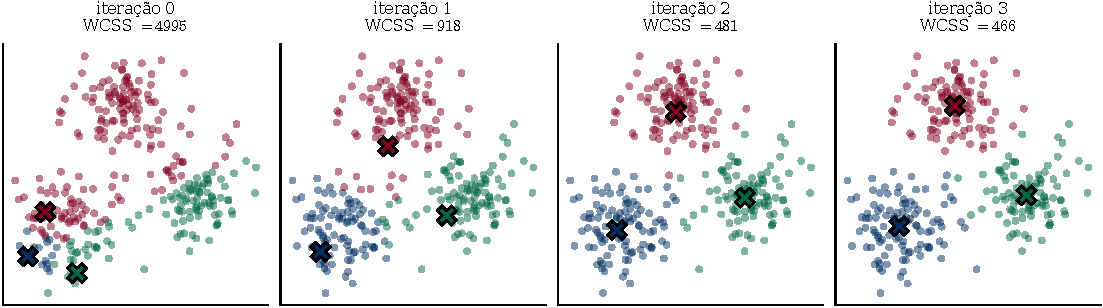
\includegraphics[width=\textwidth]{../../recursos/figuras/E1-lloyd.pdf}
  \caption{Lloyd em ação sobre $300$ pontos, partindo de uma inicialização
  deliberadamente ruim (os três centroides amontoados no canto inferior esquerdo).
  Os ``X'' são os centroides. Em três iterações eles se espalham e encontram os três
  grupos, e a WCSS cai de $4995$ para $918$, depois $481$ e $466$ --- decrescendo a
  cada passo, como a Proposição~\ref{prop:lloyd} garante, e com ganhos cada vez
  menores.}
  \label{fig:lloyd}
\end{figure}

\begin{proposicao}[Lloyd não aumenta a WCSS]\label{prop:lloyd}
Cada iteração do algoritmo de Lloyd não aumenta o objetivo \eqref{eq:wcss}; como há
finitas partições, o algoritmo converge em número finito de passos.
\end{proposicao}
\noindent\emph{Esboço.} O passo de \emph{atribuição} reduz (ou mantém) a soma das distâncias
ao centroide, pois cada ponto vai ao centroide mais próximo. O passo de
\emph{atualização} também reduz (ou mantém), pois a média é o ponto que minimiza
$\sum_{i\in C_k}\norm{\x_i-\bm{c}}^2$. Como o objetivo decresce monotonicamente e só
há finitas partições, há convergência.

\begin{atencao}
Preste atenção no que a proposição \textbf{não} diz. Ela garante que o algoritmo
\emph{para}, e que para num ponto onde nenhum dos dois passos melhora nada. Não
garante que esse ponto seja o mínimo global de \eqref{eq:wcss} --- e em geral não é.
\end{atencao}

\begin{atencao}[Mínimos locais e inicialização]
Lloyd converge para um mínimo \emph{local} que \textbf{depende da inicialização}:
sementes ruins levam a agrupamentos ruins. Soluções:
\begin{itemize}[leftmargin=1.2cm,nosep]
  \item rodar várias vezes com inícios diferentes e ficar com a menor WCSS
        (\texttt{n\_init} no \texttt{scikit-learn}) --- barato e eficaz;
  \item usar \textbf{$k$-médias++}: escolhe os centroides iniciais
        \emph{espalhados} --- o primeiro ao acaso e cada seguinte com probabilidade
        proporcional ao quadrado da distância ao centroide mais próximo já
        escolhido, $p_i\propto D^2(\x_i)$. Aumenta muito a chance de bom resultado,
        e é o padrão do \texttt{scikit-learn}.
\end{itemize}
\end{atencao}

\subsection{Escolhendo o número de grupos $K$}\label{sec:escolhaK}
$K$ é o ``\emph{tuning parameter}'', mas --- e aqui está a diferença fundamental em
relação ao resto do curso --- \textbf{sem um erro de teste para minimizar}. Não dá
para usar validação cruzada, porque não há nada contra o que validar. Restam
heurísticas:
\begin{description}[leftmargin=2.4cm,style=nextline]
  \item[Cotovelo] plote a WCSS contra $K$. Ela \emph{sempre} cai com $K$ (com $K=n$,
        WCSS $=0$), então minimizá-la é inútil; procure o ``cotovelo'', onde o ganho
        marginal despenca.
  \item[Silhueta] mede, para cada ponto, quão melhor ele se encaixa no seu grupo do
        que no grupo vizinho mais próximo. Ao contrário da WCSS, ela \emph{tem}
        máximo interior --- e por isso pode ser otimizada de fato.
\end{description}

\begin{figure}[htbp]
  \centering
  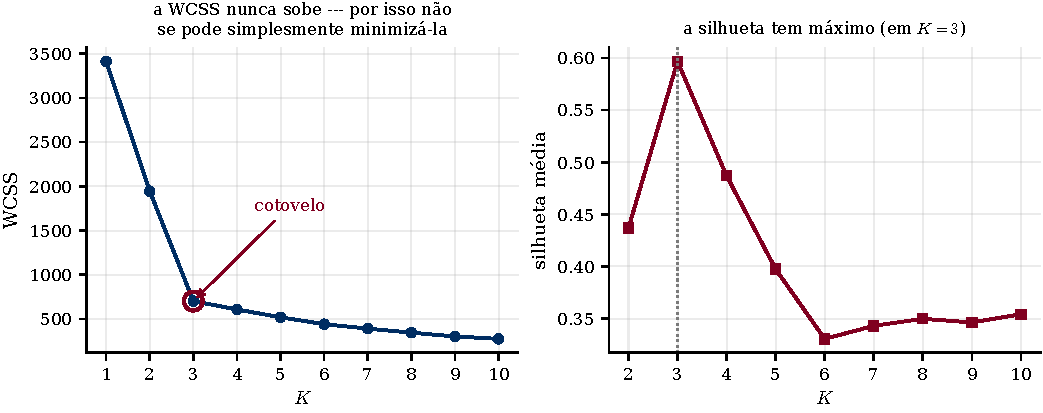
\includegraphics[width=\textwidth]{../../recursos/figuras/E1-escolha-K.pdf}
  \caption{As duas heurísticas nos mesmos dados, que \emph{de fato} têm três grupos.
  À esquerda a WCSS: ela desaba de $K=1$ a $K=3$ e depois cai devagar --- o cotovelo
  em $K=3$. À direita a silhueta média, que tem um máximo bem definido, também em
  $K=3$. Note a assimetria: o cotovelo é um julgamento visual (e nem sempre há um
  cotovelo), enquanto a silhueta dá um número.}
  \label{fig:escolhak}
\end{figure}

\begin{ideia}
Aqui está a resposta honesta à pergunta de abertura: \textbf{não existe critério
definitivo}. As duas heurísticas concordaram nesta figura porque os dados foram
gerados com três grupos bem separados. Em dados reais elas frequentemente
discordam, e nenhum dos dois números tem o \emph{status} que um erro de teste tem.
O critério final é o que a caixa lá do começo dizia: o agrupamento é bom se for
útil e interpretável no seu problema. Isso não é um defeito da técnica --- é o que
significa não ter rótulos.
\end{ideia}

\begin{exemplo}[Compressão de imagens]
Trate cada \emph{pixel} como um ponto em $\R^3$ (cores R, G, B) e rode $k$-médias
com $K$ pequeno. Substituindo cada pixel pela cor do seu centroide, a imagem passa a
usar só $K$ cores --- uma \textbf{compressão} (quantização de cor). $K$ controla a
qualidade. (É o exemplo do [AME]; compare com a compressão por SVD da Aula~E2, que
ataca o mesmo problema por outro caminho.)
\end{exemplo}

%==============================================================================
\section{Agrupamento hierárquico}
%==============================================================================
Ao contrário do $k$-médias, o agrupamento hierárquico (\emph{aglomerativo})
\textbf{não exige fixar $K$} e produz uma hierarquia de grupos:
\begin{enumerate}[leftmargin=1.6cm,nosep]
  \item comece com cada ponto em seu próprio grupo;
  \item repetidamente \emph{funda} os dois grupos mais próximos;
  \item pare quando restar um único grupo.
\end{enumerate}
O resultado é um \textbf{dendrograma} (árvore), que se ``corta'' a uma altura para
obter o número desejado de grupos. A noção de ``distância entre grupos'' é o
\emph{linkage}:
\begin{center}\small
\renewcommand{\arraystretch}{1.25}
\begin{tabular}{@{}ll@{}}
\toprule
\textbf{Linkage} & \textbf{Distância entre grupos $A$ e $B$} \\
\midrule
Completo (\emph{complete}) & $\max_{i\in A,j\in B} d(\x_i,\x_j)$ --- grupos compactos \\
Simples (\emph{single})    & $\min_{i\in A,j\in B} d(\x_i,\x_j)$ --- tende a ``encadear'' \\
Médio (\emph{average})     & média das distâncias entre pares \\
Ward                       & minimiza o aumento da WCSS na fusão \\
\bottomrule
\end{tabular}
\end{center}

\begin{figure}[htbp]
  \centering
  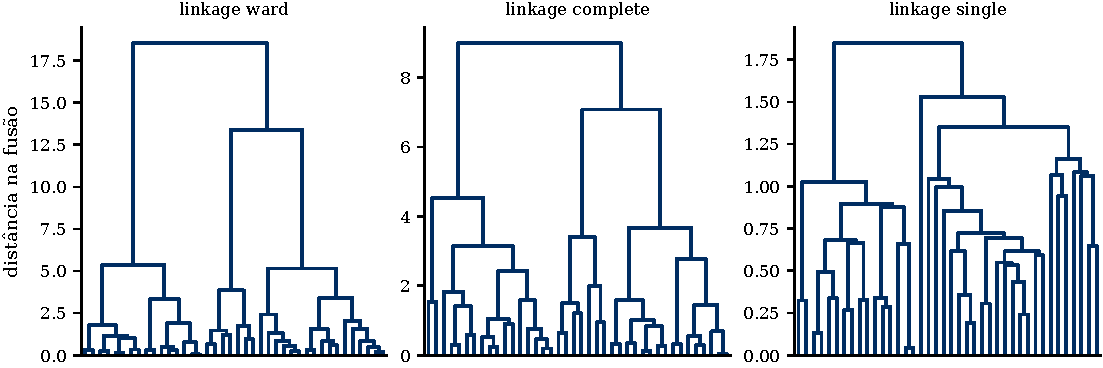
\includegraphics[width=\textwidth]{../../recursos/figuras/E1-dendrograma.pdf}
  \caption{O mesmo conjunto de $40$ pontos, três \emph{linkages}. A altura de cada
  fusão é a distância entre os grupos fundidos, e cortar o dendrograma numa altura
  dá os grupos correspondentes. Ward e completo produzem árvores equilibradas, com
  fusões altas e bem separadas --- fácil escolher onde cortar. O \emph{single}
  exibe o \emph{encadeamento} característico: ele funde repetidamente um ponto de
  cada vez ao mesmo grupo grande, porque basta \emph{um} par próximo para aproximar
  dois grupos inteiros.}
  \label{fig:dendrograma}
\end{figure}

\begin{ideia}
A vantagem do hierárquico é entregar \emph{todas} as partições de uma vez: você
decide $K$ \emph{depois} de olhar a estrutura, em vez de antes. A desvantagem é o
custo --- $O(n^2)$ de memória só para guardar as distâncias, o que o inviabiliza
com centenas de milhares de pontos, onde o $k$-médias vai bem.
\end{ideia}

%==============================================================================
\section{Prática em Python}
%==============================================================================
\begin{lstlisting}
from sklearn.cluster import KMeans, AgglomerativeClustering
from sklearn.metrics import silhouette_score
from sklearn.preprocessing import StandardScaler

X = StandardScaler().fit_transform(X)   # PADRONIZE: k-medias usa distancia

for K in range(2, 11):
    km = KMeans(n_clusters=K, n_init=10, random_state=0).fit(X)
    print(K, "WCSS:", km.inertia_, "silhueta:", silhouette_score(X, km.labels_))

# hierarquico: o dendrograma vem do scipy
from scipy.cluster.hierarchy import dendrogram, linkage
dendrogram(linkage(X, method="ward"))
\end{lstlisting}

\begin{atencao}
O \texttt{StandardScaler} não é opcional aqui, pelo mesmo motivo do KNN (Aula~04):
a distância euclidiana soma as coordenadas, e uma variável em unidades grandes
domina o agrupamento inteiro. E note que \emph{não há} \texttt{predict} honesto para
avaliar --- a diferença entre este trecho e todos os anteriores do curso é a
ausência de \texttt{y}.
\end{atencao}

Os notebooks \texttt{Aula prática E1} e \texttt{EXTRA K-medias (exemplo)} exploram o
$k$-médias, a escolha de $K$
e o efeito da inicialização.

%==============================================================================
\section*{Resumo}
%==============================================================================
\begin{itemize}[leftmargin=1.4cm]
  \item Sem rótulos não há risco a estimar: a avaliação é parcialmente subjetiva.
  \item A \emph{dissimilaridade} escolhida define o que é um grupo --- é a primeira
        decisão de modelagem, não um detalhe.
  \item \textbf{$k$-médias} minimiza a WCSS \eqref{eq:wcss}; o problema exato é
        NP-difícil e usamos o algoritmo de \textbf{Lloyd}, que converge
        (Prop.~\ref{prop:lloyd}) para um mínimo \emph{local}
        (Fig.~\ref{fig:lloyd}).
  \item Inicialização importa: use \texttt{n\_init} alto e $k$-médias++.
  \item $K$ por \emph{cotovelo} (a WCSS nunca sobe, então não se minimiza) ou por
        \emph{silhueta} (tem máximo) --- e nenhum dos dois é definitivo
        (Fig.~\ref{fig:escolhak}).
  \item \textbf{Hierárquico}: dendrograma, sem fixar $K$; o \emph{linkage} muda
        radicalmente o resultado (Fig.~\ref{fig:dendrograma}); custo $O(n^2)$.
  \item \emph{Padronize} sempre.
\end{itemize}

\paragraph{Leitura recomendada.} [AME] Capítulo~11: §11.1 ($k$-médias, com o
exemplo da compressão de imagens), §11.2 (agrupamento espectral, que não vimos aqui
e resolve casos em que o $k$-médias falha por causa da geometria dos grupos) e
§11.3 (métodos hierárquicos). [ISLP] §12.4 --- §12.4.1 ($k$-médias, com uma figura
das iterações de Lloyd equivalente à nossa Figura~\ref{fig:lloyd}), §12.4.2
(hierárquico e \emph{linkage}) e, muito recomendável, §12.4.3 (\emph{Practical
Issues in Clustering}), que discute em detalhe a fragilidade das escolhas desta
aula.

\end{document}
